\documentclass[serif]{beamer}
%\usepackage[utopia]{mathdesign}
%\usepackage[no-math]{fontspec}
%\setmainfont{Liberation Serif}

\usepackage{minted}
\usepackage{hyperref}
\usepackage{ccicons}
\usepackage{ulem}

% \usepackage{tikz}
% \usetikzlibrary{arrows,shapes,snakes,automata,backgrounds,petri}

%gets rid of bottom navigation bars
\setbeamertemplate{footline}[page number]{}

%gets rid of navigation symbols
\setbeamertemplate{navigation symbols}{}

\title{Profiling python code}
\author{Zbigniew Jędrzejewski-Szmek}
\institute{%
  
\includegraphics[width=10em]{images/Logo-redhat-color-375.png}\\
  \medskip
  \textit{zbyszek@in.waw.pl}\\
  \medskip
  \ccbysa
}
\date{\tiny Stuttgart, 2020.01.21}

\begin{document}
\begin{frame}
\titlepage % Print the title page as the first slide
\end{frame}

\begin{frame}
  \frametitle{Lecture links}

  \url{https://github.com/IMS-workshop/profiling-lecture}
\end{frame}

\begin{frame}
  \frametitle{What is optimization?}

  ``Program optimization or software optimization is the process of
  modifying a software system to make some aspect of it work more
  efficiently or use fewer resources.''

  \hfill Wikipedia
\end{frame}

\begin{frame}
  \frametitle{Premature optimization}

  ``Programmers waste enormous amounts of time thinking about, or
  worrying about, the speed of noncritical parts of their programs,
  and these attempts at efficiency actually have a strong negative
  impact when debugging and maintenance are considered. We should
  forget about small efficiencies, say about 97\% of the time:
  premature optimization is the root of all evil. Yet we should not
  pass up our opportunities in that critical 3\%.''

  \hfill Donald Knuth
\end{frame}

\begin{frame}
  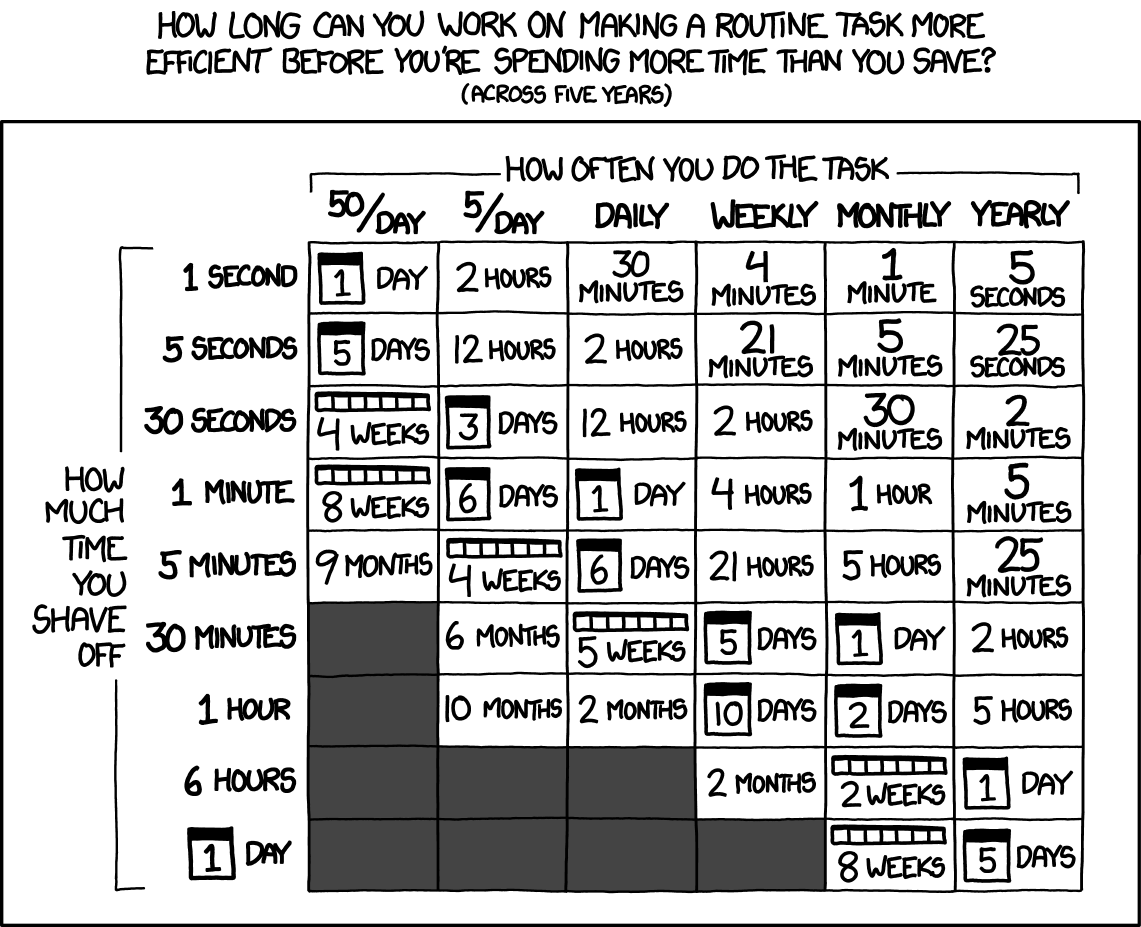
\includegraphics[width=\textwidth]{images/is_it_worth_the_time_2x.png}

  \hfill
  \href{https://xkcd.com/1205/}{xkcd.com/1205}
  
\includegraphics[height=1em]{images/240px-Cc-by-nc_icon.png}
\end{frame}

\begin{frame}
  ``Optimization is the root of all evil.''

  \hfill Donald Knuth
\end{frame}

\begin{frame}
  \frametitle{Optimization workflow}

  \begin{enumerate}
  \item \textbf{Make it work}: write the code in a simple legible way

  \item \textbf{Make it work reliably}: write automated test cases,
    make really sure that your algorithm is right and that if you
    break it, the tests will capture the breakage.

  \item Optimize the code by profiling simple use-cases to
    \textbf{find the bottlenecks} and speed up these bottlenecks,
    finding a better algorithm, or implementation.
    Keep in mind the tradeoff between simplicity and reliability
    and speed of exection of the code.
  \end{enumerate}
\end{frame}

\begin{frame}
  \frametitle{\texttt{\%timeit}}

  demo
\end{frame}

\begin{frame}
  \frametitle{Exercise}

  Please see \texttt{even-odds/exercise.txt}.

\end{frame}


\begin{frame}
  \frametitle{Exercise!}

  Make factorial faster by using a cache (e.g. a dict).

  What about \texttt{functools.lru\_cache}?
\end{frame}


\begin{frame}[fragile]
  \frametitle{\texttt{time} shell builtin}

  On *nix systems, the command time gives a quick way of measuring time:

  \begin{minted}{console}
$ time find /usr -name idontexist
1.91s user 4.32s system 36% cpu 17.279 total
    
$ time sleep 5
0.00s user 0.00s system 0% cpu 5.005 total
  \end{minted}

``total'' or ``real'' is wall clock time\\
``user'' is CPU time executing the script\\
``system'' or ``sys'' is CPU time spent in system calls
\end{frame}

\begin{frame}
  \frametitle{Exercise}

  Please see \texttt{pyc-files/exercise.txt}.

\end{frame}


\begin{frame}[fragile]
  \frametitle{\texttt{cProfile}}

  standard Python module to profile an entire application\\
  (profile is an old, slow profiling module)

  \bigskip

  Running the profiler from command line:
  \begin{minted}{console}
$ python -m cProfile -s cumtime myscript.py
  \end{minted}

  \bigskip

  Sorting options:
  \begin{itemize}
    \item
      tottime : time spent in function only
    \item
      cumtime : time spent in function and sub-calls
    \item
      calls   : number of calls
  \end{itemize}
\end{frame}

\begin{frame}[fragile]
  \frametitle{\texttt{cProfile}}

  Save results to disk:
  \begin{minted}{console}
$ python -m cProfile -o filename.prof myscript.py
  \end{minted}
  
  Explore:
  \begin{minted}{console}
$ python -m pstats filename.prof

filename.prof% help

stats [n | regexp]: print statistics
sort [cumulative, time, ...] : change sort order
callers [n | regexp]: show callers of functions
callees [n | regexp]: show callees of functions
...
  \end{minted}
\end{frame}

\begin{frame}
  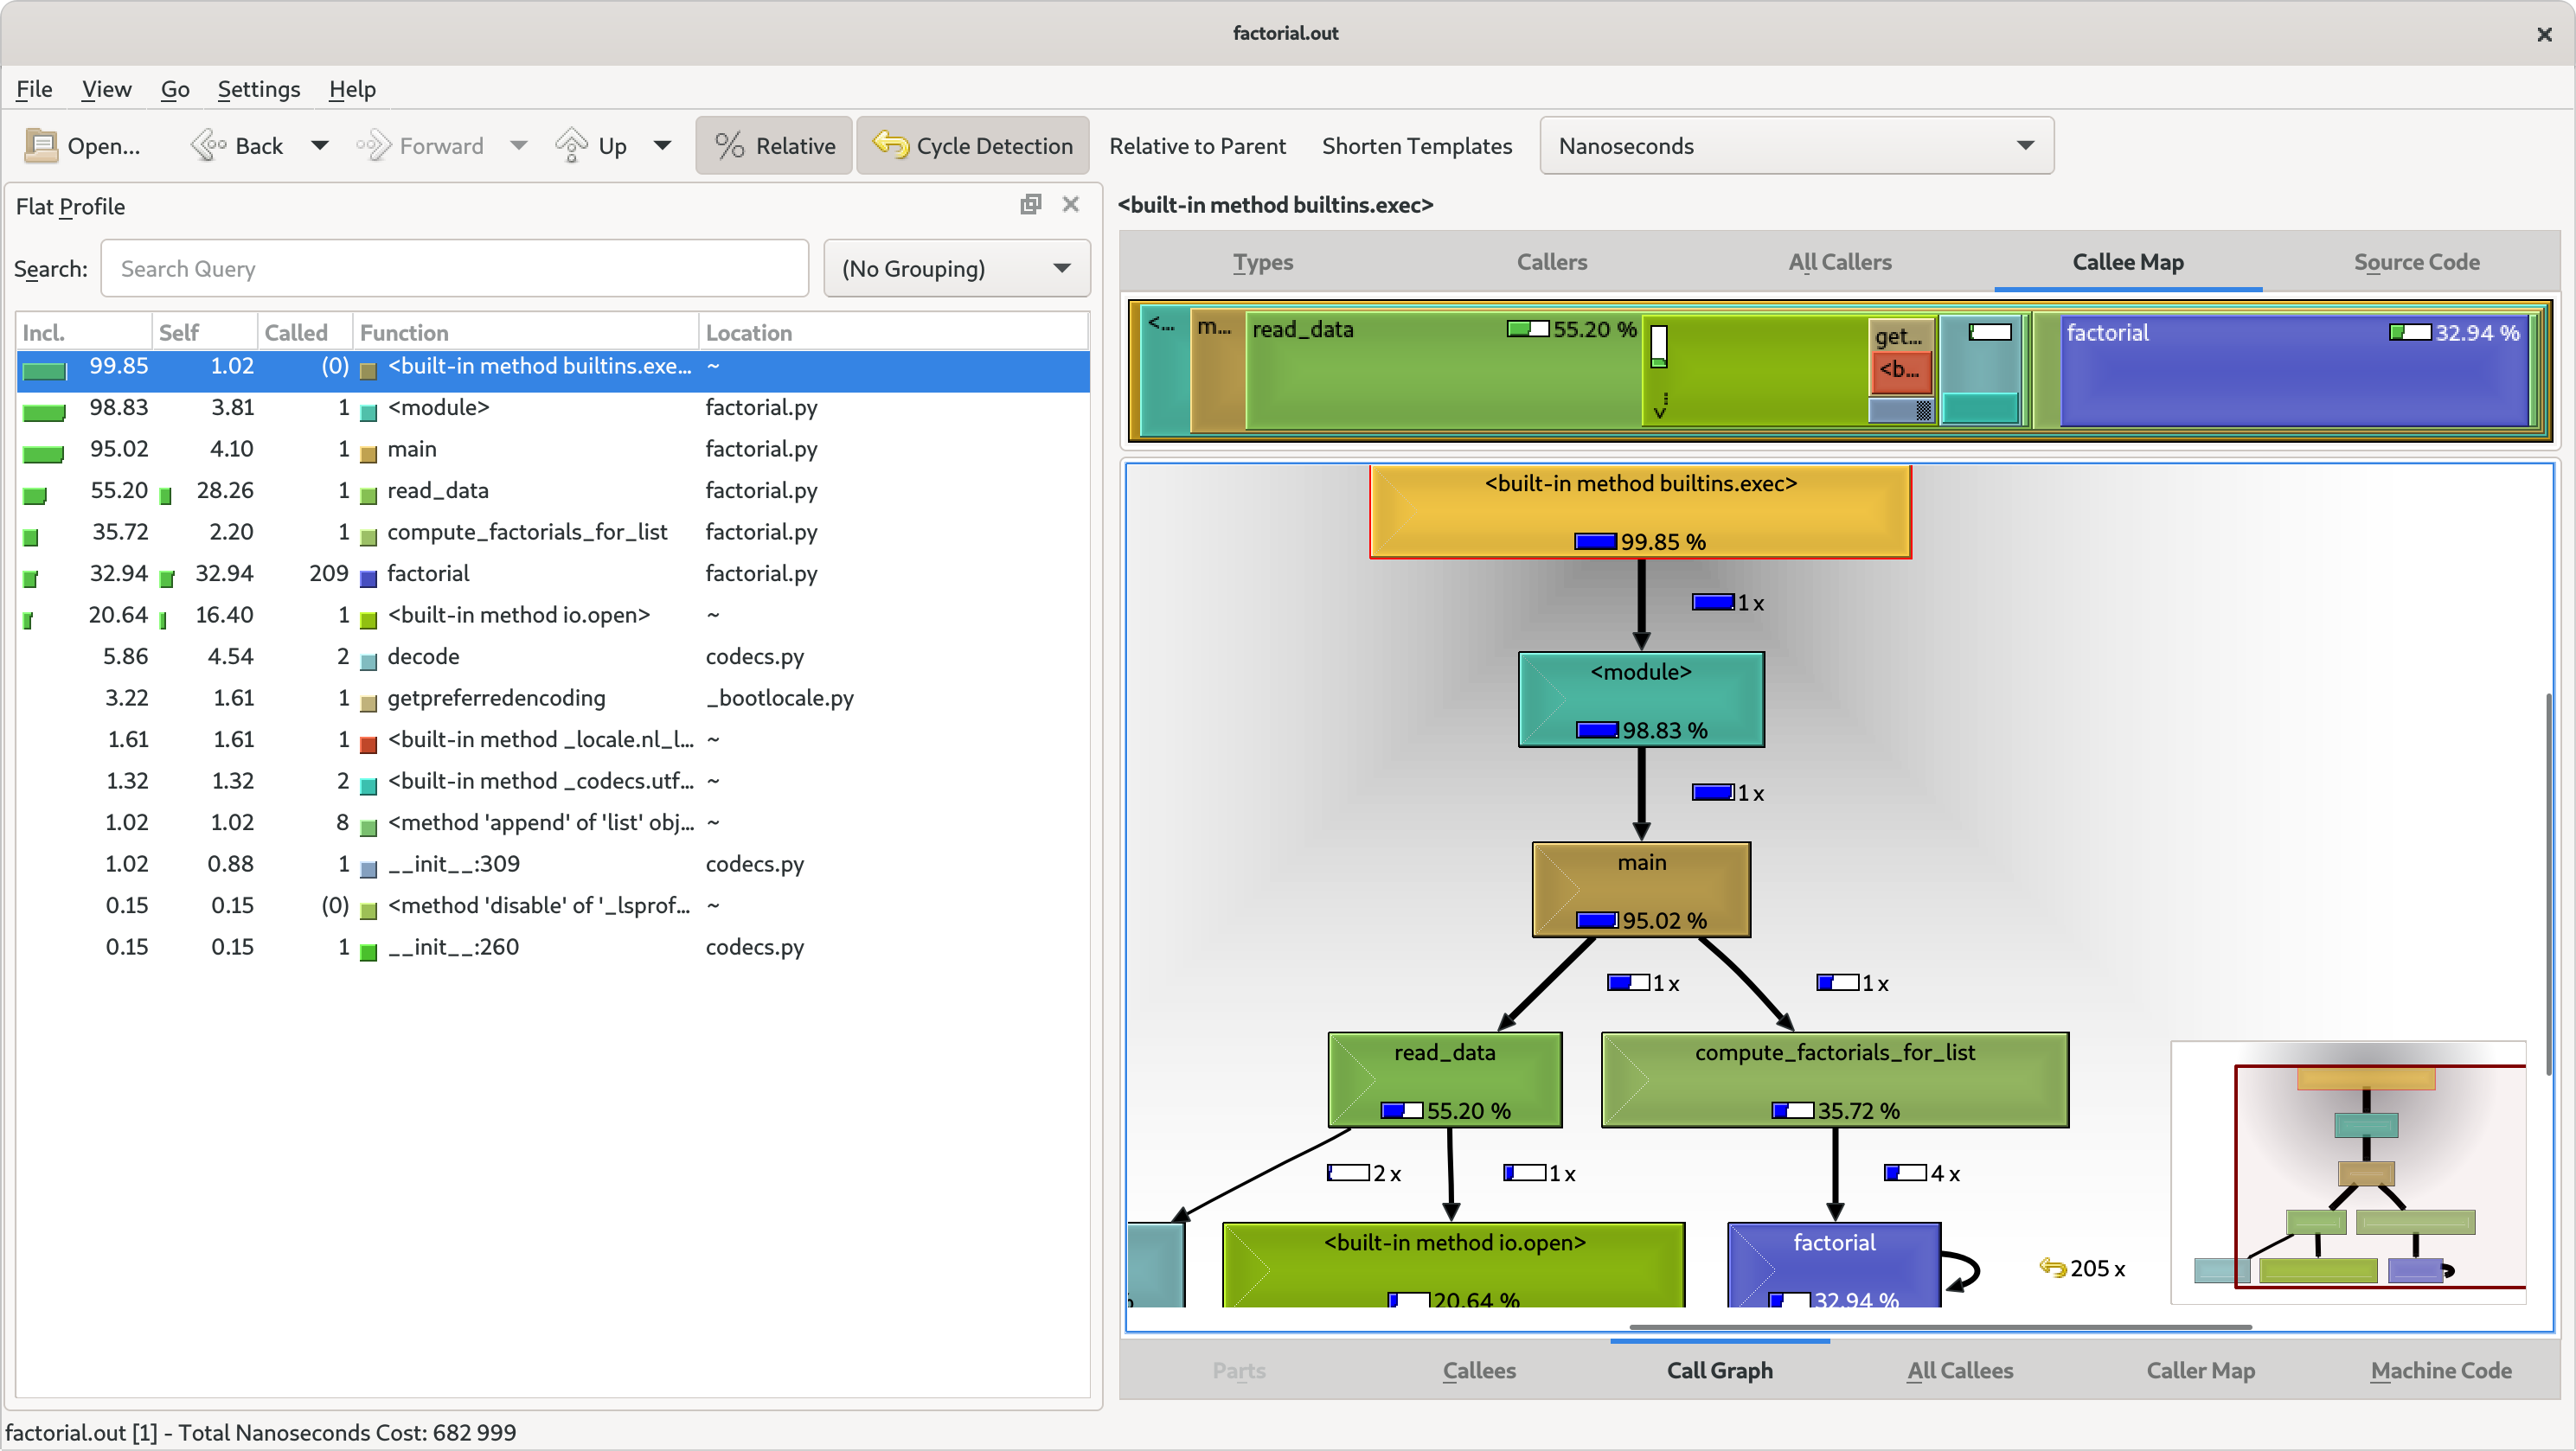
\includegraphics[width=\textwidth]{factorial/kcachegrind.png}
\end{frame}

\begin{frame}[fragile]
  \frametitle{\texttt{kernprof}}

  \begin{minted}{console}
$ sudo dnf install 'python3dist(line-profiler)'
(or)
$ pip3 install --user line_profiler
\end{minted}

  \bigskip

  \begin{minted}{python}
@profile
def slow_function(a, b, **kwargs):
    ...
  \end{minted}

  \bigskip

  \begin{minted}{console}
$ kernprof -l script_to_profile.py
$ python3 -m line_profiler script_to_profile.py.lprof
\end{minted}

\end{frame}

\begin{frame}[fragile]
  \frametitle{\texttt{pysnooper}}

  \begin{minted}{console}
$ sudo dnf install 'python3dist(pysnooper)'
(or)
$ pip3 install --user pysnooper
\end{minted}

  \bigskip

  \begin{minted}{python3}
import pysnooper

@pysnooper.snoop()
def funcition_to_trace(n):
    ...
\end{minted}

  \bigskip

\begin{minted}{console}
$ python3 script_to_trace.py |& less
\end{minted}

\end{frame}

\begin{frame}[fragile]
  \frametitle{Thanks to …}

  \begin{itemize}
  \item Pietro Berkes\\
    {\small \url{https://github.com/ASPP/testing_debugging_profiling}}
  \item Nelle Veroquaux\\
    {\small \url{https://github.com/ASPP/2019-camerino-profiling-cython-numba}}
  \end{itemize}
\end{frame}

\begin{frame}
  \frametitle{Toolbox}

  \url{https://docs.python.org/3/library/profile.html}

  \url{https://kcachegrind.github.io/}

  \url{https://github.com/rkern/line_profiler}

  \url{https://github.com/cool-RR/PySnooper}

  \url{https://pypi.python.org/pypi/memory_profiler}

  \url{http://www.camillescott.org/2013/12/06/yep/}
\end{frame}

\end{document}
